\subsection{Bipolartransistor versus Feldeffekttransistor}
	\subsubsection{Einfluss der Skalierung}
	\paragraph{Feldeffekttransistor FET}
	Ladungsträgertransport erfolgt von Source
	nach Drain. Ein FET ist ein laterales Bauelement und ist somit durch die Lithografie eingeschränkt (Kanallängen < 22nm).
	
	\todo{Ist das bei der MOS Vorlesung schon drin?}
	\paragraph{Bipolar Transistor HBT}
	Ladungsträgertransport erfolgt vom Emitter
	zum Kollektor. Ein HBT ist ein vertikales Bauelement und ist somit durch die Schichtdicke eingeschränkt (Basisdicke < 25 nm). Mehr oder weniger unabhängig von den lateralen Abmessungen.
	\subsubsection{Grundeigenschaften}
	\subsubsection{Anwendungsfelder}
	
\subsection{Bipolartransistor (Homojunktion, BJT)}
	\subsubsection{npn versus pnp}
	Der unterschied von npn und pnp Transitoren liegt im Aufbau. Die Bezeichnungen stehen dabei im direkten Zusammenhang mit der Abfolge der Schichten. So besteht der ein npn-Transistor aus zwei n-dotierten Schichten mit einer Basis aus p-dotierten Material. Der pnp-Transistor genau umgekehrt. Bei dem Schaltsymbol handelt es sich in beiden fällen um einen Strich, der von links mit der Basis (B) und von rechts mit 2 Schrägen, dem Kollektor (C) und dem Emitter (E) verbunden sind (\ref{10_npn_pnp}).  
	\begin{figure}[h]
		\centering
		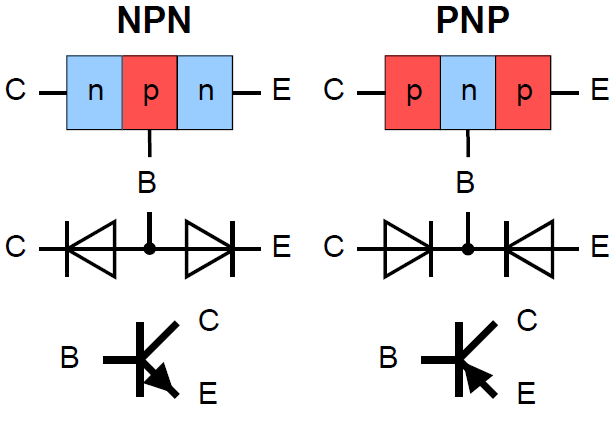
\includegraphics[width=0.4\textwidth]{Kapitel/Kap10/npn_pnp.png}
		\caption{npn- und pnp-Transistor im Vergleich}
		\label{10_npn_pnp}
	\end{figure}

	\subsubsection{Kenngrößen}
	\begin{figure}[h]
		\centering
		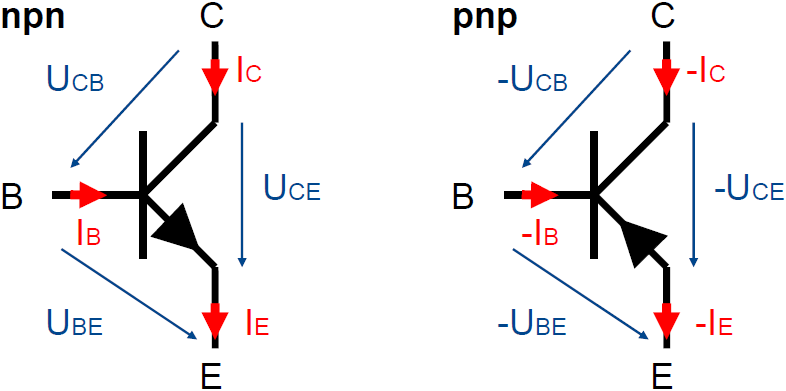
\includegraphics[width=0.4\textwidth]{Kapitel/Kap10/groessen.png}
		\caption{Unterschiedliche Kenngrößen am Bipolartransistor}
		\label{10_groessen}
	\end{figure}
	Es gibt 4 unterschiedliche Kennlinienfelder (\ref{10_kennlinie}), die einen Transistor charakterisieren.
	\paragraph{Eingangskennlinienfeld} Es wird der Basisstrom $I_B$ gegen die Basisspannung $U_{BE}$ aufgetragen. Da der Basis-Emitter Übergang als Diode gesehen werden kann, sieht diese Kennlinie wie eine Diode aus.
	\paragraph{Ausgangskennlinienfeld} Das Ausgangskennlinienfeld stellt den Kollektorstrom $I_C$ in Abhängigkeit von der Kollektor-Emitter-Spannung $U_{CE}$ und dem Basisstrom $I_B$ dar.
	\paragraph{Übertragungskennlinienfeld} Hierbei wird der Kollektorstrom $I_C$ gegen einen Basisstrom $I_B$ bei einer festgelegten Kollektor-Emitter-Spannung $U_{CE}$ aufgetragen.
	\paragraph{Spannungsrückwirkungskennlinienfeld} Dieses beschreibt die Rückwirkung der Kollektor-Emitter-Spannung $U_{CE}$ auf die Basisspannung $U_BE$ bei unterschiedlichen Basisströmen $I_B$
	\begin{figure}[h]
		\centering
		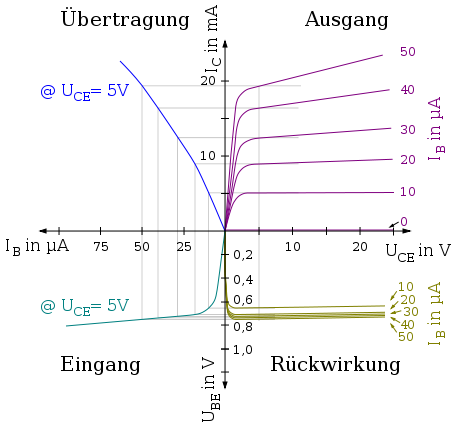
\includegraphics[width=0.6\textwidth]{Kapitel/Kap10/kennlinien.png}
		\caption{Kennlinienfelder eines Bipolartransistors}
		\label{10_kennlinie}
	\end{figure}
	  
	\subsubsection{Funktionsprinzip}
	Die drei Schichten wirken wie eine Diode. Zur Funktion muss der von Kollektor nach Emitter ein positive Spannung abfallen. Durch ein Potential an der Basis kann dann der Stromfluss auf dieser Strecke gesteuert werden.
	Im Ruhezustand bilden sich jeweils an den beiden Grenzflächen Sperrschichten aus (\ref{10_zustände} - 1). Wir nun eine positive Kollektor-Emitter-Spannung angelegt, verändern sich diese. Dabei wird die Sperrschicht zwischen Kollektor und Basis größer und zwischen Basis und Emitter kleiner (\ref{10_zustände} - 2). In diesem Zustand ist noch kein Stromfluss von Kollektor nach Emitter möglich. Wird nun noch eine gegenüber dem Emitter positive Spannung an die Basis angelegt, so kommt es zum Stromfluss (\ref{10_zustände} -3 ). Dabei ist in den Grafiken zu beachten, dass es sich bei den Spannungs- und Strom angaben um die technische, nicht die physikalische Stromrichtung handelt. Aus diesem Grund fließen die Elektronen vom Emitter zum Kollektor, obwohl die Spannung in die andere Richtung anliegt. Im letzten Zustand ist die Sperrschicht zwischen Basis und Emitter nun komplett abgebaut. Dies geschieht durch die Rekombination der Ladungen in der Basis. Diese muss sehr dünn sein, damit es nicht zu zu vielen Rekombinationen kommt. Die meisten Elektronen fließen weiter zum Kollektor (etwas 99\%).
	\begin{figure}[h]
		\centering
		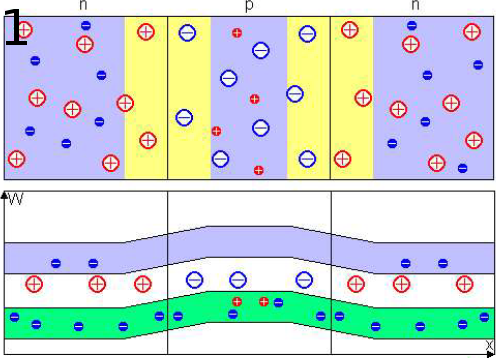
\includegraphics[width=0.4\textwidth]{Kapitel/Kap10/zustand_1.png}
		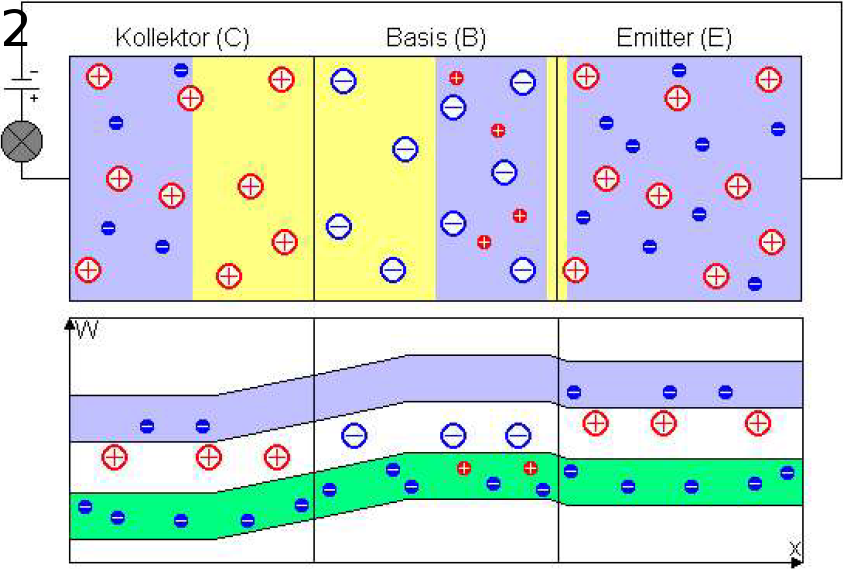
\includegraphics[width=0.4\textwidth]{Kapitel/Kap10/zustand_2.png}
		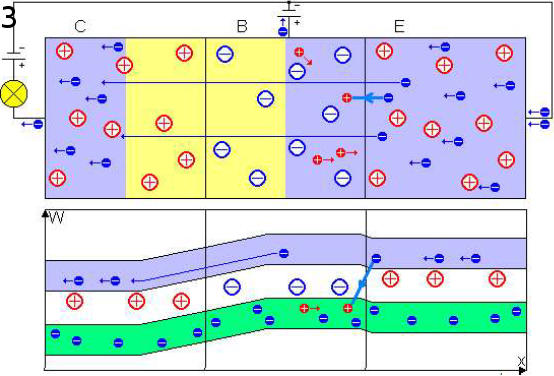
\includegraphics[width=0.4\textwidth]{Kapitel/Kap10/zustand_3.png}
		\caption{Unterschiedliche Zustande eines npn-Transistors}
		\label{10_zustände}
	\end{figure}
	Man kann nun den Kollektor und Basisstrom messen. Der Quotient beider ergibt die Stromverstärkung.
	\begin{align}
		\beta = \frac{I_C}{I_B}
		\label{10_beta}
	\end{align}
	Ein pnp-Transistor funktioniert nach dem selben Prinzip, nur sind alle Polaritäten der Strom und Spannungen umgekehrt.
	
	\paragraph{Early Effekt} Der Early-Effekt(Basisweiten-Modulation) beschreibt die Abhängigkeit des Stroms von der Kollektor-Emitter-Spannung. Wird die Spannung erhöht, so wird die Raumladungszone des Kollektor-Basis-Übergangs größer. Dementsprechend nimmt die Weite der Basis ab. Dies hat zur folge, dass man aus Transistoren keine idealen Stromquellen bauen kann. Je größer die Early-Spannung ist desto konstanter ist der Strom des Transistors.
	
	\subsubsection{Betriebsarten}
	Ein Bipolartransistor kann sich in 4 unterschiedlichen Betriebsarten befinden (\ref{10_betriebsarten}).
	\begin{table}[h]
		\centering
		\begin{tabular}{c|c|c}
			Betriebsart& EB-Übergang &CB-Übergang\\
			\hline
			Sättigung & Fluss & Fluss\\
			Aktiv (Normal) & Fluss & Sperr\\
			Invertiert & Sperr & Fluss\\
			Sperrbetrieb & Sperr & Sperr
		\end{tabular}
		\caption{Unterschiedliche Betriebsarten des Bipolartransistors}
		\label{10_betriebsarten}
	\end{table}
	\paragraph{Sperrbereich} Beide Übergänge sperren. Theoretisch stell dies einen offenen Schalter dar, dementsprechend sollte kein Strom fließen, allerdings gibt es geringe Leckströme. Der Transistor ist somit kein idealer Schalter.
	\paragraph{Aktiv} Dieser Bereich wird auch Normalbetrieb oder Verstärkerbereich genannt. Die Emitterdiode ist in Flussrichtung und die Kollektordiode in Sperrrichtung. Näherungsweise gilt die Formel für die Stromverstärkung (\ref{10_beta}). Der Transistor wird üblicherweise nur so betrieben, das diese Verstärkung über die Stromänderung annähernd konstant bleibt. 
	\paragraph{Sättigung} In diesem Bereich leiten beide Dioden. Die Basis enthält allerdings mehr Ladungsträger als notwendig, welche beim ausschalten zunächst abtransportiert werden müssen. In diesem Bereich verhält sich der Transistor wie ein Schalter mit konstanten Durchgangswiderstand.
	\paragraph{Invertiert} In diesem, auch inverser Verstärkerbereich, genannten Zustand ist der Basis-Kollektor-Übergang in Durchlassrichtung und der Basis-Emitter-Übergang in Sperrrichtung. Alles funktioniert hier wie im normalen Verstärkerbereich, allerdings ist die Stromverstärkung wesentlich geringer. 
	\subsubsection{Grundschaltungen}
\subsection{Heterojunktion Bipolartransistor (HBT)}
	\subsubsection{Aufbau}
	\subsubsection{Vorteile gegenüber BJT}
	\subsubsection{Erreichbare Leistungen}
	\subsubsection{Modulare Integration}


\todo{Fragen aus Own Clowd zuordnen}
\todo{Gruppenübungs-Inhalte ergänzen}